\documentclass{article}

\usepackage{amsmath, amsthm, amssymb, latexsym, amsfonts}
\usepackage{comment, enumerate, mathrsfs, stmaryrd, hyperref}
\usepackage{tikz}
\usepackage{xcolor}
\usepackage{graphicx}
\usepackage{titlesec}
\usepackage{blindtext}
\usepackage[a4paper, total={7in, 9in}]{geometry}

\begin{document}

\begin{titlepage}
    \begin{center}
        \vspace*{0.6cm}
            
        \Huge
        \textbf{Do you like Texas hold 'em}
            
        \vspace{0.5cm}
        \LARGE
        STAT230 Real World Assignment 2024W
            
        \vspace{1.5cm}
            
        \textbf{Eason Li, Johnson Ji}
            
        \vspace{3.6cm}
        
        \begin{center}
            
\includegraphics[width = 0.4\textwidth]{UofLoo.png}
        \end{center}

        \vspace{0.4cm}
            
        \Large
        Falculty of Math \\
        University of Waterloo \\
        Canada \\
        April 8, 2024
    \end{center}
\end{titlepage}

\newpage

\begin{center}
    \textcolor{blue}{
        In this report, we consider the case a player uses the best 
        five-card poker hand out of seven cards.
    }
\end{center}

For a 7-card hand to contain a Royal Flush, it must contain the specific 
set of 5 cards (Ace, King, Queen, Jack, 10 of the same suit), with the 
other 2 cards being any of the remaining 47 cards in the deck. Since the 
Royal Flush can come from any of the four suits, and the two additional 
cards can be any other two cards from the remaining 47, the number of 
ways to get a Royal Flush in a 7-card hand is the product of the number 
of suits (4) and the number of combinations of the remaining 47 cards 
taken 2 at a time, which is $C(47,2)$.

\[
P(\text{Royal Flush in 7-card poker}) = \frac{4 \times C(47, 2)}{C(52, 7)}
\]

\begin{center}
    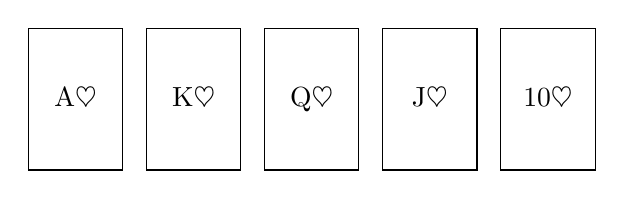
\begin{tikzpicture}
        \foreach \rank/\suit/\x in {A/\(\heartsuit\)/0, K/\(\heartsuit\)/1.5, Q/\(\heartsuit\)/3, J/\(\heartsuit\)/4.5, 10/\(\heartsuit\)/6} {
        % Draw the card
        \draw (\x,0) rectangle ++(1.2,1.8);
        % Add the rank and suit
        \node at (\x+0.6,0.9) {\rank\suit};
        }
    \end{tikzpicture}
\end{center}






\end{document}
